\documentclass[11pt, oneside]{article}   	% use "amsart" instead of "article" for AMSLaTeX format
\usepackage{geometry}                		% See geometry.pdf to learn the layout options. There are lots.
\geometry{letterpaper}                   		% ... or a4paper or a5paper or ... 
%\geometry{landscape}                		% Activate for for rotated page geometry
%\usepackage[parfill]{parskip}    		% Activate to begin paragraphs with an empty line rather than an indent
\usepackage{graphicx}				% Use pdf, png, jpg, or eps� with pdflatex; use eps in DVI mode
								% TeX will automatically convert eps --> pdf in pdflatex		
\usepackage{amssymb}
\usepackage{amsmath}
\usepackage{parskip}
\usepackage{hyperref}

\title{Logarithm and Exponential Functions}
%\author{The Author}
%\section{}
% \section*{R code}
\date{}							% Activate to display a given date or no date

\graphicspath{{/Users/telliott_admin/Dropbox/Tex/png/}}

\begin{document}
\maketitle
\noindent
\Large
\section{Introduction}

The logarithm and exponential functions are inverses.  If we have that
\[ y = b^x \]
for some $b > 0, b \ne 1$, then we say that
\[ x = \log_b \ y \]
Putting them together
\[ y = b^{\ \log_b y} \]
The usual bases are $10$ (common logarithm, $\log_{10}$, or just $\log$), $e$ (natural logarithm or $\ln$), and $2$ (binary logarithm or $\log_2$).

The rules for exponents are simple, if $p$ and $q$ are two numbers and we know the logarithms of $p$ and $q$ to base $b$
\[ p = b^{u}; \ \ \ q = b^{v} \]
then their product can be computed as:
\[ pq = b^{u + v} \]
provided we can actually compute $b^{u+v}$.  In the old days there were tables of logarithms, so you just looked up the answer in the table.

The second rule is that:
\[ (b^u)^v = b^{uv} \] 
And in terms of logarithms we write
\[ \log_b (b^u)^v = \log b^{uv} = v \log_b (b^u) \]

For example 
\[ 2^2 = 2 \times 2 = 4 \] 
\[ 2^3 = 2 \times 2 \times 2 = 8 \]
\[ 4 \times 8 = 2^2 \times 2^3 = 2^{2 + 3} = 2^5 \]
\[ = 2 \times  2 \times 2 \times 2 \times 2 = 32 \]
and
\[ (2^2)^3 = 4^3 = 64 = 2^6 = 2^{2 \times 3} \]

Here is a plot of $\log_{10}(x)$ and $\ln x$:
\begin{center} 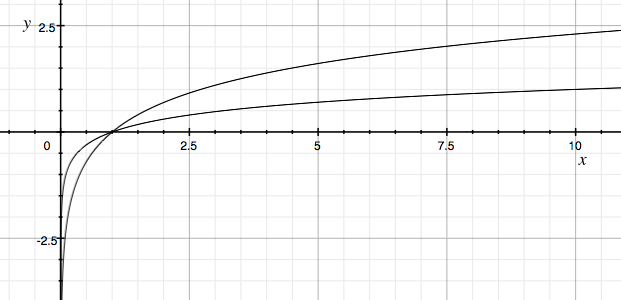
\includegraphics [scale=0.5] {log1.png} \end{center}
The first function reaches the value $1$ when $x=10$ and the second reaches the value $1$ when $x=e$.  Both have the value $0$ at $x=1$ because $b^0 = 1$ for any base, so the logarithm to any base of $1$ is equal to $0$.

Since
\[ x \ \frac{1}{x} = 1 \]
\[ \log ( x \cdot \frac{1}{x} ) = \log 1 = 0 \]
so
\[ \log x + \log \frac{1}{x} = 0 \]
\[ - \log x = \log \frac{1}{x} \]

It turns out that if we take the logarithm of $x$ (where $x$ is any number $> 1$) to two \emph{different} bases, the ratio of the logarithms is a constant, independent of the value of $x$.  This is best shown by the change of bases formula.
\[ \log_b n = \frac{\log_a n}{\log_a b} \]

Start with
\[ y = b^x \]
\[ x = \log_b y \]
Take logarithms to the base $a$:
\[ \log_a y = \log_a (b^x) \]
Using the second rule
\[ \log_a y = x \log_a b \]
Substitute for $x$
\[ \log_a y = \log_b y \log_a b \]
Rearranging:
\[ \log_b y = \frac{\log_a y}{\log_a b} \]
$y$ can be any value, so replace it by $x$
\[ \log_b x = \frac{\log_a x}{\log_a b} \]
The way I remember this is that first
\[ \log_b x = k \log_a x \]
the logarithms to different bases are connected by some constant $k$, and we substitute for $k$ the inverse of the log to the \emph{same} base as we have in the numerator:
\[ \log_b x = \frac{\log_a x}{\log_a b} \]
Alternatively, you might look at the other formula
\[ \log_b x \log_a b = \log_a x  \]
and think of the $b$'s canceling in some way (not that they do, of course).

One other thing we can do is to set $x=a$ in the above formula.  We start from
\[ \log_b x = \frac{\log_a x}{\log_a b} \]
then with $x=a$
\[ \log_b a = \frac{\log_a a}{\log_a b} \]
but $\log_a a = 1$ so
\[ \log_b a = \frac{1}{\log_a b} \]

And that makes perfect sense.  If we multiply by some factor $c$ to convert from the logarithm in base $a$ to base $b$, we must multiply by the inverse the same factor to convert back again.

For the figure above of the common log (base 10) and the natural logarithm, $\ln 10 = 2.303$, and that looks about right, when $x=10$ the first function is $1.0$ and the second one is about $2.3$.

The logarithm and the exponential are inverse functions, we can see that if we plot them together:
\begin{center} 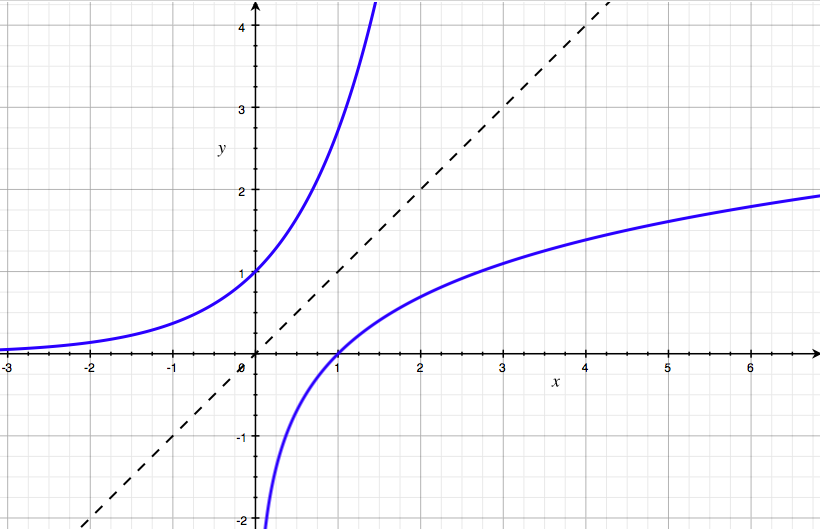
\includegraphics [scale=0.5] {log2.png} \end{center}
The upper curve is $y = e^x$ and the lower one is $y = \ln x$.
As inverse functions, they are symmetric about the line $y=x$.  Also, if we consider an $x$ value, for example $x=1$, then the slope of the curve $y=e^x$ at $x=1$ (at the point $(1,e)$) is the inverse of the slope of the curve $y=log(x)$ when $x=e$ (at the point $(e,1)$).

\section{Fractional Exponents}
The introduction above dealt mainly with integer exponents, but of course you know that the practical use of logarithms depends on fractional values.  The simplest way to see how this works is to consider the square root.
\[ \sqrt{2} \times \sqrt{2} = 2 \]
If we think about what the exponent $u$ to the base $2$ would be such that
\[ 2^u = \sqrt{2} \]
We observe that by the rules for exponents
\[ \sqrt{2} \times \sqrt{2} = 2^u \times 2^u = 2^{u+u} = 2^1 \]
That is
\[ u + u = 1 \]
so $u = 1/2$.  By the same logic the $n^{\text{th}}$ root of $b$ is $b^{1/n}$.  And of course 
\[ (b^2)^{1/2} = b^{2 \times 1/2} = b^1 \]
Feynman has a nice description of how logarithms were calculated (see Lectures, volume 1, Chapter 22, Algebra;  
\url{http://www.feynmanlectures.caltech.edu/I_22.html}).
The basic idea is to take repeated square roots of the base ($10$), and then combine those to form the required value.
\section {$x < 1$}

Fractional exponents leads to consideration of $0 < x < 1$.  Write
\[ x \ \frac{1}{x} = 1 \]
Take the logarithm of both sides
\[ \log(x \ \frac{1}{x} ) = \log 1 = 0 \]
\[ = \log x + \log \frac{1}{x} \]
Thus
\[ \log \frac{1}{x} = - \log x \]

\section{Principal and interest}
Suppose I put $100$ dollars in the bank, and the people at the bank say that after one year, they will give me an additional $\$10$ at that time.  We say that they are paying $10\%$ interest for the year on the principal $P$ of $\$100$.

However, suppose I bargain with them.  I get them to promise to pay me half the interest ($5\%$) at the six-month mark, and the rest after one year.  My account will hold $\$105$ after six months, and the interest due for the second half will be $5\%$ of $\$105$, which is $\$5.25$ for a total of $\$10.25$.

The equation to describe this is that if the rate of interest is $r$ and the year is broken up into $n$ periods when interest will be paid, the total amount at the end will be:
\[ A = P(1 + \frac{r}{n})^n \]
This is compound interest.  If there are additional years $t$, the exponent will be $nt$ rather than $n$.

Now it turns out, as we will see below, that 
\[ (1+b)^{mn} = (1+bm)^n \]
It is a little counter-intuitive, but nevertheless true.  So in the equation
\[ A = P(1 + \frac{r}{n})^n \]
the same factor can be either in the second term inside or up in the exponent.  So we bring out the factor $r$ and obtain
\[ A = P(1 + \frac{1}{n})^{nr} \]
\[ A = P \ [ \ (1 + \frac{1}{n})^{n} \ ] ^r \]
And now we start wondering what happens if the bank pays every month $r=12$ or every day $r=365$ or every second.  What happens if the interest is compounded continuously?
\[ A = \lim_{n \rightarrow \infty} P \ [ \ (1 + \frac{1}{n})^{n} \ ] ^r \]

This becomes the question, what is the value
\[ A = \lim_{n \rightarrow \infty} (1 + \frac{1}{n})^{n} \]
It is going to turn out that this limit is equal to a number which is called $e$
\[ e = 2.71828\ 18284\ 59045 \dots \]

\section{Difference quotient for exponential}
We'll start the calculus part of this by looking at what happens to an exponential function when we vary $x$ by a small amount $h$.  We want
\[ \lim_{h \rightarrow 0} \frac{b^{x+h} - b^x}{h} \]
for some base $b$.  We can rewrite this as
\[ \lim_{h \rightarrow 0} \frac{b^{x}b^{h} - b^x}{h} \]
\[ \lim_{h \rightarrow 0} \frac{b^{x}(b^{h}-1)}{h} \]
Now, the thing is that $b^x$ does not depend on $h$, so it doesn't change as we go to the limit, and thus we have
\[ b^x \lim_{h \rightarrow 0} \frac{b^{h}-1}{h} \]
We don't know what the term under the limit is equal to yet, but it is not dependent on $x$, so it is a constant.  Therefore, the slope of the exponential
\[ y = b^x \]
for some base $b$ is
\[ y' = cb^x \]
The slope is the same as the function, up to a constant.  (It turns out that if $b=e$, then $c=1$ and we will have:
\[ y = e^x \]
\[ y' = e^x \]
The function $e^x$ is its own derivative, which leads to all of its amazing properties.  We can easily calculate the value of the limit
\[ \lim_{h \rightarrow 0} \frac{b^{h}-1}{h} \]

Set $h=0.00001$ and use Python.  For the following values of $b$ I get:
\[ b=2  \rightarrow 0.693 \]
\[ b = 2.71828 = e \rightarrow 1.000  \]
\[ b = 10 \rightarrow 2.302 \]
This is one \emph{definition} of $e$.

It will not surprise you to learn that these values correspond to the natural logarithm of the base.

So $e$ is the value for which
\[ \lim_{h \rightarrow 0} \frac{e^{h}-1}{h} = 1 \]
We can rearrange the limit as follows:
\[ \lim_{h \rightarrow 0} e^{h} = 1 + h \]
\[ \lim_{h \rightarrow 0} e = (1 + h)^{1/h} \]
This can also be written as
\[ \lim_{x \rightarrow \infty} e = (1 + \frac{1}{x})^{x} \]

This can be calculated using Python, but it doesn't converge so fast.  For $x=100000$, I get $e = 2.718168$, which is only correct to 4 places.

\section{evaluating the limit}
We can use the binomial theorem to evaluate 
\[ \lim_{x \rightarrow \infty} e = (1 + \frac{1}{x})^{x} \]
and show that it is equivalent to
\[ e = \frac{1}{0!} + \frac{1}{1!} + \frac{1}{2!} + \frac{1}{3!} + \cdots  \]

which is yet another one of the equivalent definitions for $e$.  The first three terms are $1 + 1 + 1/2$, which is reasonably close. After six terms, we have $e = 2.718$.  The series converges rapidly because the inverse factorials get small very quickly.  (See below).

We will do that, but as an alternative, I saw an interesting approach to this in the book \emph{Mooculus}.  We will use L'Hopital's Rule.  We're looking for
\[ \lim_{x \rightarrow \infty} \ (1 + \frac{1}{x})^x \]
the first thing is to rewrite this as the exponential
\[ 1 + \frac{1}{x} = e^{\ln(1 + 1/x)} \]
and then
\[ (1 + \frac{1}{x})^x =  (e^{\ln(1 + 1/x)})^x = \ e^{x \ln(1 + 1/x)} \]
To evaluate the limit, we need to evaluate the limit of the exponent
\[ \lim_{x \rightarrow \infty} x   \ln (1 + \frac{1}{x})  \]

At first, it doesn't look like we can use L'Hopital's Rule (there is no quotient), but there is a standard trick for these situations.  Just rearrange like so
\[ = \lim_{x \rightarrow \infty} \frac{ \ln (1 + \frac{1}{x})}{\frac{1}{x}}  \]
Both the top and the bottom limits are easily evaluated to be equal to $0$.  So now we will differentiate.  The derivative of the numerator is (by the chain rule)
\[ f'(x) = \frac{-x^{-2}}{1 + 1/x} \]
while the denominator is just
\[ g'(x) = -x^{-2} \]

So we need to evaluate
\[ = \lim_{x \rightarrow \infty} \frac{f'(x)}{g'(x)} \]
The factor of $-x^{-2}$ cancels from both top and bottom, leaving us with
\[ = \lim_{x \rightarrow \infty} \frac{1}{1 + 1/x} = 1  \]
Substituting back, we see that
\[ \lim_{x \rightarrow \infty} \ (1 + \frac{1}{x})^x \]
\[ = \lim_{x \rightarrow \infty} \  e^{x \ln(1 + 1/x)} \]
\[ = e^1 = e \]

\section{Using the binomial theorem}
Evaluating 
\[ \lim_{x \rightarrow \infty} e = (1 + \frac{1}{x})^{x} \]

If we use the standard binomial expansion
\[ \frac{1}{0!}a^n + \frac{n}{1!}a^{n-1}b^1 + \frac{n(n-1)}{2!}a^{n-2}b^2 + \frac{n(n-1)(n-2)}{3!}a^{n-3}b^3\ + \cdots \]
with a = 1
\[ \frac{1}{0!} + \frac{n}{1!}b^1 + \frac{n(n-1)}{2!}b^2 + \frac{n(n-1)(n-2)}{3!}b^3\ + \cdots \]
plug in for b = 1/n
\[ \frac{1}{0!}({\frac{1}{n}})^0 + + \frac{n}{1!}({\frac{1}{n}})^1 + \frac{n(n-1)}{2!}({\frac{1}{n}})^2 + \frac{n(n-1)(n-2)}{3!}({\frac{1}{n}})^3 + \cdots  \]
Now, in the limit as $x \rightarrow \infty$, $n$ and $n-1$ are nearly equal, and so are $n$ and $n-2$, and all the terms $n$, $(n-1)$, $(n-2)$ find just the right number of $n$'s in the denominator to cancel and we get
\[ \frac{1}{0!} + \frac{1}{1!} + \frac{1}{2!} + \frac{1}{3!} + \cdots  \]
which is one of the definitions we gave above for $e$, and evaluated as $e = 2.718$.  

So $e$ is just a number.  We can define the exponential function, which means we raise $e$ to the power $x$, that is $f(x) = e^x$.  We have
\[ e = \lim_{n \to \infty} (1 + \frac{1}{n})^{n} \]
We want 
\[ e^x = \lim_{n \to \infty} (1 + \frac{1}{n})^{nx} \]
It turns out this is exactly the same as
\[ e^x = \lim_{n \to \infty} (1 + \frac{x}{n})^{n} \]

It seems counterintuitive.  But the result follows from
\[ (1+b)^{mn} = (1+mb)^n \]
To confirm this, look at the binomial expansion for these two expressions.  Remember that the terms $n(n-1)(n-2)(n-3)$ etc. come from this formula
\[ \frac{n!}{(n-k)!k!} \]
so for example, with $k=3$ we have
\[ n! = n \times (n-1) \times (n-2) \times (n-3)! \]
\[  \frac{n!}{(n-k)!k!} = \frac{n(n-1)(n-2)(n-3)!}{(n-3)!\ 3!} \]
\[ = \frac{n(n-1)(n-2)}{3!} \]

Thus, in the first one
\[ e^x = \lim_{n \to \infty} (1 + \frac{1}{n})^{nx} \]
With $nx$ as the exponent, the factorial part is
\[ \frac{(nx)!}{((nx)-k)!\ k!} \]
so for example the $k=3$ term is
\[ \frac{nx \times (nx-1) \times (nx-2)}{3!} \]

we get a power of $nx$ coming in for each term in the numerator
\[ \frac{1}{0!}({\frac{1}{n}})^0 + + \frac{nx}{1!}({\frac{1}{n}})^1 + \frac{nx(nx-1)}{2!}({\frac{1}{n}})^2 + \frac{nx(nx-1)(nx-2)}{3!}({\frac{1}{n}})^3 + \cdots  \]
The subtracted value of $k$ is negligible in the limit, and the $n$'s cancel as before but the $x$'s do not, so that gives finally
\[ e^x = \frac{x^0}{0!} + \frac{x^1}{1!} + \frac{x^2}{2!} + \frac{x^3}{3!} + \dots \]

Now, the second version is
\[ \lim_{n \to \infty} (1 + \frac{x}{n})^{n} \]

\[ \frac{1}{0!}(\frac{x}{n})^0 + + \frac{n}{1!}({\frac{x}{n}})^1 + \frac{n(n-1)}{3!}({\frac{x}{n}})^2 + \frac{n(n-1)(n-2)}{3!}({\frac{x}{n}})^3 + \cdots  \]

The $n$'s cancel as before and we have
\[ e^x = \frac{x^0}{0!} + \frac{x^1}{1!} + \frac{x^2}{2!} + \frac{x^3}{3!} + \cdots \]
\[= 1 + x + \frac{x^2}{2!} + \frac{x^3}{3!} + \cdots  \]
Note:  this assumes that the binomial applies to fractional exponents, which is a bit complicated to show.

Also note that a very useful approximation for small $x$ is
\[ e^x \approx 1 + x \]

If you need more precision, you can add another term:
\[ e^x \approx 1 + x + \frac{x^2}{2!} \]

\section{The exponential is its own derivative}

A most important fact about the exponential function $f(x) = e^x$ is that this function is its own derivative.  To see that, take $\frac{d}{dx}$ of the last series.
\[ \frac{d}{dx} \ e^x = 0 + (1)\frac{x^{1-1}}{1!} + (2)\frac{x^{2-1}}{2!} + (3)\frac{x^{3-1}}{3!} + \cdots  \]
\[ \frac{d}{dx} \ e^x = 0 + \frac{x^{0}}{0!} + \frac{x^{1}}{1!} + \frac{x^{2}}{2!} + \cdots  \]
\[ = e^x \]
Each exponent $n$ that comes down through the power rule, finds an $n$ in $n!=n \times (n-1) \times (n-2) \dots $ to cancel, leaving $n-1$ in the exponent as well as $(n-1)!$.

We can find the derivative of a generic exponential using the standard method with the difference quotient.  Let $b$ be the base, then $f(x) = b^x$ and
\[ \lim_{h \to 0}    \ \frac{b^{x+h} - b^x}{h}   \]
But
\[  b^{x+h} = b^x b^h  \]
so this is just
\[ \lim_{h \to 0}    \ \frac{b^xb^h - b^h}{h} \]
\[ = \lim_{h \to 0}    \ \frac{b^x(b^h - 1)}{h} \]
\[ = b^x  \lim_{h \to 0}\ \frac{(b^h - 1)}{h} = cb^x \]

We didn't ever say exactly what the value of $c$ is, just that it is just a number which depends on b, but \emph{not on x}, so we know it's a constant.  It turns out that 
\[ c = \log_b e \]

So if $b = e$, then $c=1$.  You can see that by looking at
\[ \lim_{h \to 0}\ \frac{(e^h - 1)}{h} \]
For small $h$ we can approximate $e^h = 1 + h$ (see the series above), then
\[ \lim_{h \to 0}\ \frac{(1 + h - 1)}{h} = \frac{h}{h} = 1 \]

\section{one problem}
I don't have a lot of problems in this write-up but I will put two here about integration of the exponential.  Since 
\[ \frac{d}{dx} e^x = e^x \]
and by the chain rule
\[ \frac{d}{dx} e^{f(x)} = e^{f(x)} f'(x) \]
And generally, for $u = u(x)$ have that 
\[ \int e^u \ du = e^u + C \]
So what is 
\[ \int x e^x \ dx \]
The systematic approach uses integration by parts, but we can get there by just playing with the derivative
\[ \frac{d}{dx} \ x e^x = x e^x + e^x \]
so 
\[ \int \frac{d}{dx} \ x e^x \ dx = \int x e^x \ dx + \int e^x \ dx \]
\[ x e^x = \int x e^x \ dx + e^x \] 
\[ \int x e^x \ dx = x e^x - e^x \] 
The second one requires a special trick.  
\[ \int_0^{\infty} \frac{1}{1 + e^x} \ dx \]
Multiply by $e^{-x}$ on top and bottom
\[ \int_0^{\infty} \frac{e^{-x}}{1 + e^{-x}} \ dx \]
This is just $\int 1/u \ du$.  Remember the minus sign
\[ = - \ln (1 + e^{-x}) \ \bigg |_0^{\infty} \]
At the upper limit we obtain $\ln 1 = 0$ and at the lower limit we have 
\[ - - \ln 2 = \ln 2 \]
so
\[ \int_0^{\infty} \frac{1}{1 + e^x} \ dx = \ln 2 \]

\section{from exponential to logarithm}
It is possible to obtain the definition of the derivative of the logarithm from:
\[ \int \frac{1}{t} \ dt = \ln(t) \]
\[ \frac{d}{dt} \int \frac{1}{t} \ dt  = \frac{1}{t}  = \frac{d}{dt} \ln(t) \]
This is great because we never did generate $x^{-1}$ by differentiating powers of $x$.  Now we know how to go back the other way.  

The proof is so simple that if you blink, you'll miss it.  Again, we found that the exponential function is its own derivative.  That is
\[ y = e^x \]
\[ \frac{d}{dx} e^x = \frac{dy}{dx} = e^x  \]
\[ \frac{dy}{dx} = y \]
Invert
\[ \frac{dx}{dy} = \frac{1}{y} \]
\[ dx = \frac{1}{y} \ dy \]
Integrate
\[ \int dx = x = \int \frac{1}{y} \ dy \]
And what is $x$?  It is $\ln(y)$!
\[ \ln(y) = \int \frac{1}{y} \ dy \]
And since $y$ is just a letter, we can write the same for $x$, or $t$
\[ \ln(t) = \int \frac{1}{t} \ dt \]
One of the prettiest things I've ever seen.

The math purists don't like it, but in general it is OK to do algebra with differentials.  One important restriction is that $dy/dx$ (and $dx/dy$) should not be equal to zero.  And a second one is that we just remember we are never passing to the limit, just getting really, really, really close.  (As close as you like).

Now that we have this definition, we have another way of estimating the value of $e$.  We add up the areas for little slices under the function $y=1/x$ until we reach $1$.  That value of $x=e$.
\begin{center}
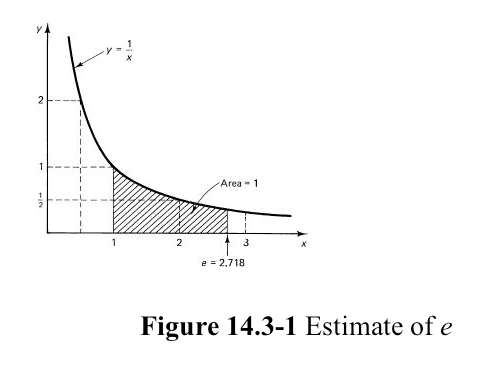
\includegraphics [scale=0.6] {log3.png}
\end{center}
(from Hamming's \emph{Calculus}).

For example, we might try intervals of $0.1$ and do
\[ 0.1 \cdot \frac{1}{1} + 0.1 \cdot \frac{1}{1.1} + 0.1 \cdot \frac{1}{1.2} + \dots + 0.1 \cdot \frac{1}{2.7} \]
I tried this in Python, but it didn't work so well.  (Need to figure this out).

\section{reverse direction}
As we said above, differentiating both sides of the last equation we get
\[ {\frac{d}{dx} \ln(x) = \frac{1}{x} } \]
We want to go backward now, to show that the derivative of the function $f(x) = e^x$ is itself.  Start with
\[ \ln(e^x) = x \]
\[ \frac{d}{dx} \ln(e^x) = \frac{d}{dx} x = 1 \]
but using the property we just proved and the chain rule, this is also
\[ \frac{d}{dx} \ln(e^x) = \frac{1}{e^x} \ \frac{d}{dx} e^x  \]
so these two expressions are equal and
\[ \frac{1}{e^x} \ \frac{d}{dx} e^x = 1  \] 
\[ \frac{d}{dx} e^x = e^x \]

\section{half-life}
A sample of radioactive phosphate containing the isotope ${}^{32}$P decays with a half-life of just over 14 days (14.29, to be more precise).  If you want to solve a problem with a given amount of the chemical $N_o$ at time-zero ($t=0$), and you are asked for the amount at time $t$, what do you do?  If the time is an even multiple of the half-life, it's easy.  For one half-life, multiply by $\frac{1}{2}$, for two half-lives multiply by $\frac{1}{4}$, for $n$ half-lives multiply by $(\frac{1}{2})^n$.

If the time is not an even multiple of the half-life, you need two equations (where $T$ is the half-life and $k$ is a rate constant)
\[ kT = \ln 2  = 0.693 \]
\[ N = N_o \ e^{-kt} \]

I want to show where these equations come from.  When studying the exponential function in calculus, we learn two equivalent definitions.  The first is that $\frac{d}{dx} \ e^x = e^x$.  The second is that $\frac{d}{dx} \ \ln(x) = \frac{1}{x}$, or 
\[ \int \frac{1}{x} \ dx = \ln(x) \]

In radioactive decay, each atom has a fixed probability of disintegrating in the next short time interval $dt$.  The probability varies for different types of radioactive atom (${}^{3}$H, ${}^{14}$C, ${}^{238}$U, etc.), but for each phosphorus atom in our sample of ${}^{32}$P it is the same.  As a result, the number of atoms $dN$ that will disintegrate or decay in the short time $dt$ is proportional to $N$, the number currently present.  A fixed fraction of all the atoms will be transformed.  We write
\[ dN = k N dt \]
Rearrange and integrate
\[ \int \frac{dN}{N} = \int k \ dt \]
The answer is just
\[ \ln(N) = kt + C_0 \]
Form the exponential on both sides
\[ N = Ce^kt \]
($C = e^{C_0}$).  We evaluate the constant $C$ by setting $t=0$ and find that $C = N_o$ so
\[ N = N_o \ e^{kt} \]
Finally, for decay problems it is usual to let $k$ be positive and introduce a minus sign
\[ N = N_o \ e^{-kt} \]
The other equation given above was
\[ kT = \ln 2 = 0.693 \]

This is very useful to remember, because frequently we are given a half-life $T$ and asked to compute using the  equation with $e^{-kt}$.  It will save time to convert $T$ to $k$ quickly.  

The derivation is as follows.  By definition, after one half-life has elapsed, when the time $t = T$, $N = N_o/2$.
\[ \frac{N_o}{2} = N_o \ e^{-kT} \]
\[ \frac{1}{2} =  \ e^{-kT} \]
\[ 2 =  \ e^{kT} \]
\[ \ln 2 =  \ kT \]

Equations for the growth of populations work similarly, with 
\[ N = N_o \ e^{kt} \]
and again, if the problem gives you an even number of doublings, or generations, just use that.  For growth equations it is usual to use another symbol like $g$ for the number of generations, where
\[ N = 2N_o \ e^{kg} \]
but the same relation holds between $g$ and $k$ (because of the switched minus sign in $e^{kt}$).
\[ \ln 2 =  \ kg \]

\section{from logarithm to exponential}
In more advanced treatments (what the math guys call analysis), it becomes a bit harder to introduce the exponential and logarithm in a natural way. 

What they do is to investigate a particular function often called $L$, and show that the function $L$ has all the properties of the logarithm, \emph{so it is the logarithm}.  Then we will go backwards from the logarithm to the other properties of $e$, like its value, and the fact the its derivative is itself.

This approach comes straight from David Jerrison's lecture in Calculus 1 (MIT online course).  We define the logarithm function as

\[ L(x) = \int_1^x \frac{dt}{t} \]
\begin{center}
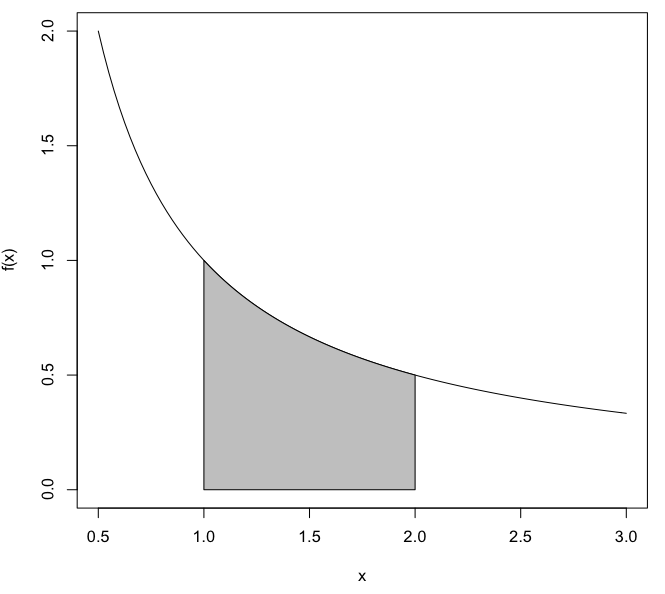
\includegraphics [scale=0.45] {inv.png}
\end{center}
For example, the logarithm of $2$ is the area under the curve above, $f(x) = 1/x$, between $ 1 \le x \le 2$.  Having defined
\[ L(x) = \int_1^x \frac{dt}{t} \]

By the Fundamental Theorem of Calculus (part II) we have
\vspace{2 mm}

\noindent Property 1
\[ L'(x) = \frac{1}{x} \]
The slope of the logarithm function is always positive ($x>0$), but is undefined for $x=0$
\begin{center}
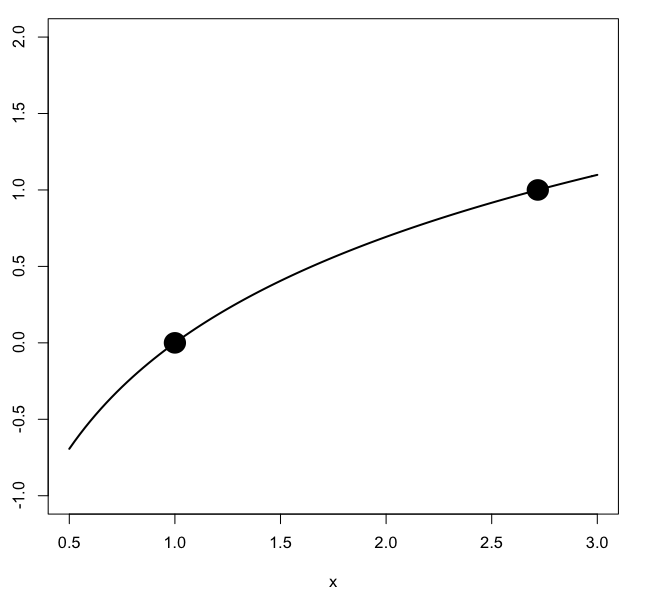
\includegraphics [scale=0.45] {log.png}
\end{center}
\vspace{2 mm}

\noindent Property 2
\[ L(1) = \int_1^1 \frac{dt}{t} = 0 \]
This property is by definition.  It fits with our use of exponents, where $b^0 = 1$.
\vspace{2 mm}

\noindent Property 3
\[ L''(x) = - \frac{1}{x^2} \]
Although the area under the curve $ln(x)$ is always increasing, so the slope is always positive, the rate of increase of the slope is always decreasing, so the shape is concave down.
\vspace{2 mm}

\noindent Property 4
\[ L(e) = 1 \]
This is by definition as well.  In extending to exponents it means we can write $y = ln(x) \iff e^y = x$.
\vspace{2 mm}

\noindent Property 5
\[ L(ab) = L(a) + L(b)  \]
To show that this last statement is true involves showing that this is equivalent
\[ \int_1^{ab} \frac{dt}{t} = \int_1^{a} \frac{dt}{t} + \int_a^{ab} \frac{dt}{t} \]
For the arguments $a$ and $ab$ we have 
\[ L(ab) = \int_1^{ab} \frac{dt}{t}   \]
\[ L(a) = \int_1^{a} \frac{dt}{t}   \]
Both of these are true by definition.  The one that takes a little work is
\[ L(b) = \int_a^{ab} \frac{dt}{t}   \]
Substitute $au=t$, then $a \ du = dt$ and
\[ L(b) = \int \frac{a \ du}{au} = \int \frac{du}{u}  \]
with a change in the limits
\[ t=a \Rightarrow u=1  \]
\[ t=ab \Rightarrow u=b  \]
So it's just
\[ L(b) = \int_1^b \frac{du}{u}  \]
which is again, true by definition.  So the function $L$ has the property that $L(ab) = L(a) + L(b)$, which is one of the two major properties of logarithms.

To see that the second is also true, start with
\[ L(a^r) = \int_1^{a^r} \frac{dt}{t}   \]
Substitute $t=u^r$, so $dt = ru^{r-1} du$, and the limits become 
\[ t=1 \Rightarrow u=1  \]
\[ t=a^r \Rightarrow u=a  \]
\[ L(a^r) = \int_{t=1}^{t=a^r} \frac{dt}{t} = \int_{u=1}^{u=a} \frac{1}{u^r} (ru^{r-1}) du = r \int_{u=1}^{u=a}  \frac{du}{u} = rL(a) \]
As Dunham says (using A for L) "these properties of the hyperbolic area---namely $A(ab) = A(a) + A(b)$ and $A(a^r) = rA(a)$---exactly mirror the corresponding properties of logarithms.  Clearly something interesting is afoot."

\section{Difference quotient for logarithm}
As seen in Hamming's \emph{Methods of Mathematics Applied to Calculus, Probability and Statistics}, we can also go back to the definition of the logarithm as the reverse of the exponential
\[ f(x) = \log_b x \]
and write the difference quotient
\[ f'(x) = \lim_{h \rightarrow 0}  \frac{\log_b (x + h) - \log_b x}{h}  \]
and then rearrange it as follows:
\[ =  \lim_{h \rightarrow 0} \frac{\log_b (\frac{x+h}{x})}{h} \]
\[ =  \lim_{h \rightarrow 0} \frac{\log_b (1 + \frac{h}{x})}{h} \]
\[ =  \lim_{h \rightarrow 0} \log_b \ [ \ (1 + \frac{h}{x})^{1/h} \ ]  \]
\[ =  \lim_{h \rightarrow 0} \frac{1}{x}  \ [ \ ( \log_b (1 + \frac{h}{x})^{x/h}  \ ]  \]
\[ =   \frac{1}{x}  \ \lim_{h \rightarrow 0}  \ [ \ ( \log_b (1 + \frac{h}{x})^{x/h}  \ ]  \]

So it's clear that we will need to evaluate the term for which we are taking the logarithm, in the limit
\[ =  \lim_{h \rightarrow 0} (1 + \frac{h}{x})^{x/h} \]
Let $t = h/x$.  Then this becomes
\[ =  \lim_{t \rightarrow 0} (1 + t)^{1/t} \]
which ought to look familar (section 5).  It is one of the definitions of $e$.  We have then that
\[ \frac{d}{dx} \log_b x = \frac{1}{x} \ \log_b e \]
If we use the natural logarithm, then we have
\[ \frac{d}{dx} \ln x = \frac{1}{x} \ \ln e = \frac{1}{x} \]

There is another derivation which is essentially identical to this one in videos on Khan Academy.

\section{another version (showing that $e$ is equal to a limit)}
In this section, we demonstrate that the number $e$ is equivalent to a limit:
\[ \lim_{n \rightarrow \infty} (1 + \frac{1}{n})^n \]

I am simply following the proof as I found it online 

(here:  \url{http://aleph0.clarku.edu/~djoyce/ma122/elimit.pdf }).

So we start with a different definition of $e$ and show that it is equivalent.  We begin with this definition of the natural logarithm:
\[ \ln x = \int_1^x \frac{1}{t} \ dt \]

We have worked through some consequences above, following David Jerrison's MIT lecture.  It can be shown fairly easily that this function has all the properties of the natural logarithm.

In addition to that definition, we need two more properties, first:
\[ \ln 1 = \int_1^1 \frac{1}{t} \ dt = 0 \]

fairly obvious, since the upper and lower bounds are equal, and then second, our definition of $e$.  It is the number such that
\[ \ln e = \int_1^e \frac{1}{t} \ dt = 1 \]

So here's the proof.  Let $t$ be any number in an interval $[1, 1 + 1/n]$.  We're interested in what happens as $n$ gets large.  We have that
\[ 1 \le t \le 1 + \frac{1}{n} \]

If we invert each term, then $\le$ becomes $\ge$, but we will instead rearrange the terms:
\[ \frac{1}{1 + \frac{1}{n}} \le \frac{1}{t} \le 1 \]

The only tricky step is this one:  for each of the above, we integrate the variable $t$ between the endpoints $1$ and $1 + 1/n$, remembering that $n$ is just a number and so is $1 + 1/n$, so we have
\[ \int_1^{1 + 1/n} \frac{1}{1 + \frac{1}{n}} \ dt \le \int_1^{1 + 1/n} \frac{1}{t} \ dt \le \int_1^{1 + 1/n}  1 \ dt \]

The first integral is a constant times $t$ evaluated between $1 + 1/n$ and $1$ which is equal to the constant times $1/n$:
\[ \ [ \ \frac{1}{1 + \frac{1}{n}} \ ] \  \frac{1}{n} = \frac{1}{1 + n} \]

The second one is $\ln (1 + 1/n)$ by the definition of the logarithm, and the third is the same integral as the first but without the constant, so we have that:
\[ \frac{1}{1 + n} \le \ln (1 + \frac{1}{n} ) \le \frac{1}{n} \]

From here on, we just rearrange things a bit.  Exponentiating each term doesn't change the inequality:
\[ e^{1/1 + n} \le 1 + \frac{1}{n} \le e^{1/n}\]

The left-hand inequality can be raised to the power $(n+1)$ giving:
\[ e \le (1 + \frac{1}{n})^{n + 1} \]

and divide by $ (1 + \frac{1}{n})$
\[ \frac{e}{1 + 1/n} \le (1 + \frac{1}{n})^{n} \]

We notice that, in the limit as $n \rightarrow \infty$, this becomes 
\[ e \le  \lim_{n \rightarrow \infty} (1 + \frac{1}{n})^n \]

Similarly for the right-hand inequality, raise to the power $n$ giving:
\[ (1 + \frac{1}{n})^{n} \le e \]

and in the limit as $n \rightarrow \infty$, this becomes
\[ \lim_{n \rightarrow \infty} (1 + \frac{1}{n})^{n} \le e \]

Call the limit $L$.

The only way that $e \le L$ and $L \le e$ can both be true is if $e$ is equal to the limit in question.  This is the squeeze theorem.  Hence
\[ e = \lim_{n \rightarrow \infty} (1 + \frac{1}{n})^n \]

\section{some useful results}
Now that we know that 
\[ \ln x = \int \frac{1}{x} \ dx \]
\[ \frac{d}{dx} \ln x = \frac{1}{x} \]
we can extend this using the chain rule
\[ \frac{d}{dx} \ln (f(x)) = \frac{1}{f(x)} \ f'(x) \]

One new problem that we can solve using this is 
\[ \frac{d}{dx} x^x \]
The standard methods don't work for this one.  Take the logarithm:

\[ \ln (x^x) = x \ln x \]
Now, take the derivative of both sides.  The left-hand side is
\[ \frac{d}{dx} \ln f(x) = \frac{f'(x)}{f(x)} = \frac{f'(x)}{x^x} \]
The right-hand side is just
\[ \frac{d}{dx} x \ln x = x \frac{1}{x} + \ln x = 1 + \ln x \]
So putting it together
\[ f'(x) = \frac{d}{dx} x^x = x^x (1 + \ln x) \]

Another useful result is to prove the power rule.  We want
\[ \frac{d}{dx} x^n \]
where $n$ is not just a positive or negative integer ($\ne -1$), but can be a real number, like $\pi$ or $e$ or $\sqrt{2}$.

Take the logarithm
\[ \ln x^n = n \ln x \]
\[ \frac{d}{dx} f(x) = \frac{f'(x)}{f(x)} \]
\[ = \frac{d}{dx} n \ln x = n \frac{1}{x} \]
So
\[ f'(x) = \frac{d}{dx} x^n =   n \ \frac{1}{x} \ x^n = n x^{n-1} \]

It is somewhat less interesting, but logarithmic differentiation can be used to solve problems that would otherwise be quite unwieldy
\[ \frac{d}{dx} \ [ \ \frac{x^9 e^{4x}}{\sqrt{x^2 + 4}} \ ] \]
We could write this as
\[ \frac{f(x) g(x)}{h(x)} \]
And solve it using the product rule and the quotient rule.  Or we can take the logarithm
\[ \ln f(x) = \ln x^9 + \ln e^{4x} - \ln \sqrt{x^2 + 4} \]
\[ = 9 \ln x + 4x - \frac{1}{2} \ln (x^2 + 4) \]
and then take the derivative
\[ \frac{9}{x} + 4 - \frac{x}{(x^2 + 4)} \]
and then apply the rule:
\[ \frac{d}{dx} \ln f(x) = \frac{f'(x)}{f(x)} \]
So we multiply by $f(x)$ to obtain the result:
\[ f'(x) = ( \frac{9}{x} + 4 - \frac{x}{(x^2 + 4)}) \  \frac{x^9 e^{4x}}{\sqrt{x^2 + 4}} \]
which would obviously be a real mess by the standard approach.

\section{maximum likelihood}

One more nice example is of a set of Bernoulli trials, like a series of coin flips where the coin isn't fair, but instead has a probability $p$ of coming up heads (H) and $1-p$ of coming up tails (T).  

Now, $p$ is unknown, but we have some data about how the coin performs, and we wish to use the data to estimate $p$ by the method of maximum likelihood.  We observe this sequence of trials:
\[ HTHHTTTHTHHH \]

Theory says that the probability of observing this sequence of events is dependent on $p$ in the following way:
\[ p(1-p)pp(1-p)(1-p)(1-p)p(1-p)ppp = p^7(1-p)^5 \]

We call the probability of observing this data, \emph{given} some underlying probability model $p$, the likelihood $L$:
\[ L(p) = p^7(1-p)^5 \]

And in general, since each trial is independent and identically distributed, we can write that for $n$ trials and $k$ successes we would have
\[ L(p) = p^k(1-p)^{n-k} \]

Here, $n$ and $k$ are constants for any particular sequence, but we would like to have the general formula.
 
To find the maximum for $L$ we differentiate and set that equal to 0.
\[ \frac{d}{dp} L = 0 \]
However, we note that since $\ln L$ increases and decreases along with $L$, the $p$ that gives a maximum for $L$ also gives a maximum for $\ln L$, and we will set:
\[ \frac{d}{dp} \ln L = 0 \]
\[ \ln L = k \ln p + (n-k) \ln(1-p) \]
Take the derivative $d/dp$ of both sides (we get a minus sign from the chain rule):
\[ \frac{d}{dp} L = 0 = \frac{k}{p} - \frac{n-k}{1-p} \]
Rearrange, then multiply through by $1-p$ and also by $1/k$:
\[ \frac{1-p}{p} = \frac{n-k}{k} \]
\[ \frac{1}{p} = \frac{n}{k} \]
\[ p = \frac{k}{n} \]
As we might have thought, the best guess for $p$ is the observed number of successes in that many trials, $k/n$.

\section{A connection to sine and cosine}
Recall that starting from this definition
\[ \frac{d}{dx} e^x = e^x \]
we were able to prove that
\[ \frac{d}{dx} \ln x = \frac{1}{x} \]

Euler said, let us consider the complex number
\[ z = \cos \theta + i \sin \theta \]
How did he come up with this?  Because he already knew the answer, I guess.  Let's just see what we can do.  If we assume that calculus is legal with complex numbers (since $i$ is \emph{just a number}), we can do the following
\[ \frac{dz}{d \theta} = - \sin \theta + i \cos \theta \]

And since $i*i = -1$
\[ \frac{dz}{d \theta} = i*i \sin \theta + i \cos \theta \]
\[ \frac{dz}{d \theta} = i(i \sin \theta + \cos \theta) \]
\[ \frac{dz}{d \theta} = iz \]

Rearrange
\[ \frac{1}{z} dz = i d \theta \]
\[ \int \frac{1}{z} dz = \int i d \theta \]
\[ \ln z = i \theta \]
Exponentiate:
\[ z = e^{i \theta} \]
\[ e^{i \theta} = \cos \theta + i \sin \theta \]

Euler's famous result, which he proved more rigorously by different approaches.
Let's use it to get something useful for calculus.  Switch notation to $s$ and $t$

\[ e^{i s} = \cos s + i \sin s \]
\[ e^{i t} = \cos t + i \sin t \]
\[ e^{i (s+t)} = \cos (s+t) + i \sin (s+t) \]
But
\[ e^{i (s+t)} = e^{i s} e^{i t} \]
\[ = (\cos s + i \sin s) \ (\cos t + i \sin t) \]
\[ = \cos s \cos t + \cos s i \sin t + i \sin s \cos t - \sin s \sin t \]
\[ = (\cos s \cos t - \sin s \sin t) + i (\sin s \cos t + \cos s \sin t ) \]
So we have an equality between two complex numbers, both equal to $e^{i (s+t)}$.  For this to be true, both the real and imaginary parts must be equal.

\[ \cos (s+t) = \cos s \cos t - \sin s \sin t \]
\[ \sin (s+t) = \sin s \cos t + \cos s \sin t \]
The addition formulas for sine and cosine.

\section{Improper integral and volume}

The log function provides a fun example of an improper integral with a very simple and finite result.  The example (and the figure) are from Hamming.
\begin{center} 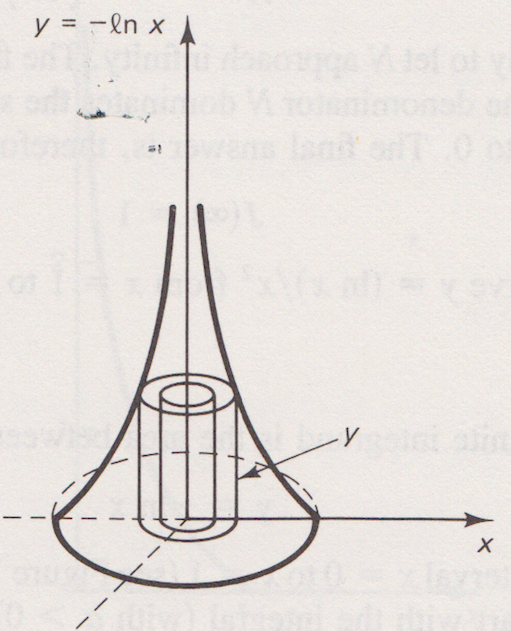
\includegraphics [scale=0.4] {log4.png} \end{center}
We consider the function
\[ y = - \ln x = \ln \frac{1}{x} \]
(section 3)

We use the minus sign so we are working with positive $y$, recognizing that the function is not defined as $x=0$.  Rotate the function around the $y$ axis and find the volume.

To use the method of cylinders, we consider a series of concentric cylindrical surfaces of width $dx$, ranging from $x=0$ to $x=1$.  For each value of $x$, the surface area is the height of the function $h = - \ln x$ times the circumference $2 \pi x$ to give a volume for each element of
\[ dV = 2 \pi x y \ dx = 2 \pi x (- \ln x) \ dx \]
We get the total volume by integrating
\[ V = \int_0^1 2 \pi x (- \ln x) \ dx \]

What is $\int x \ln x \ dx $?  The systematic approach is to use integration by parts, but let's guess.  If we had $f(x) = x^2 \ln x$ then part of the derivative $f'(x)$ would be related to what we want:
\[ \frac{d}{dx} x^2 \ln x = 2 x \ln x + \dots \]
So we'll go ahead and fill it in if we can
\[ \frac{d}{dx} x^2 \ln x = 2 x \ln x + \frac{x^2}{x} = 2 x \ln x + x \]
we add a factor of $1/2$ and another term of $-x^2/2$
\[ f(x) = \frac{1}{2} ( x^2 \ln x - \frac{x^2}{2} ) \]
\[ f'(x) = \frac{1}{2} ( 2 x \ln x + x - x ) = x \ln x \]
So
\[ \int x \ln x \ dx =  \frac{1}{2} ( x^2 \ln x - \frac{x^2}{2} ) \]
The volume $V$ is equal to $-2 \pi$ times
\[ \frac{1}{2} ( x^2 \ln x - \frac{x^2}{2} ) \bigg |_0^1 \]
At the upper limit, $\ln 1 = 0$ so this is $-1/4$, and the question becomes, what happens to $x^2 \ln x$ as $x$ approaches $0$?  We guess that $x^2$ must become small faster than $\ln x$ approaches $-\infty$.  So at the lower limit, we will get zero, and the whole thing is
\[ V = -2 \pi \ (-\frac{1}{4}) = \frac{\pi}{2} \]

Let's try by the method of disks and then come back to this limit.  We also have a figure for the second approach
\begin{center} 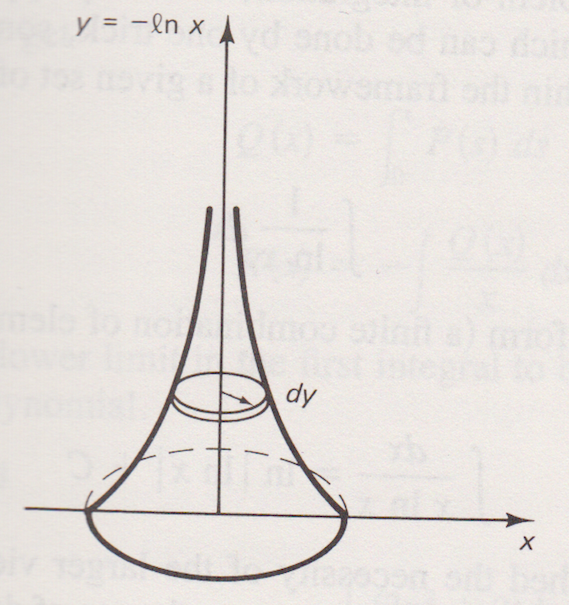
\includegraphics [scale=0.4] {log5.png} \end{center}
As $y$ ranges from $0$ to $\infty$, each disk has a width $dy$ and an area equal to $\pi x^2$ so the volume element is
\[ dV = \pi x^2 \ dy \]
We change variables and write
\[ y = - \ln x \]
\[ dy = - \frac{1}{x} \ dx \]
so
\[ dV = - \pi x^2 \ \frac{1}{x} \ dx = - \pi x \ dx \]
The limits also change.  Before we had $y = 0 \rightarrow \infty$ and now we have $x = 1 \rightarrow 0$ so
\[ V = \int_1^0 - \pi x \ dx \]
\[ = \pi \int_0^1 x dx \]
\[ = \frac{\pi}{2} x^2 \ \bigg |_0^1 =  \frac{\pi}{2} \]

So it looks like we were right about that limit.  But what is the formal method for evaluating
\[ \lim_{x \rightarrow 0} x^2 \ln x \]
We convert this to a fraction
\[ \lim_{x \rightarrow 0} \frac{\ln x}{1/x^{2}} \]
Since both numerator and the denominator go to $\infty$ as $x \rightarrow 0$, this is an indeterminate form, and we can use L'Hopital's rule.  We need derivatives of the numerator and the denominator.  The numerator gives $1/x$ and the denominator gives $-2/x^{3}$ so we have
\[ \frac{1}{x} \ \frac{1}{-2/x^{-3}} = \frac{x^3}{x}(- \frac{1}{2}) = - \frac{x^2}{2} \]
which in the limit as $x \rightarrow 0$, also goes to $0$.

Generally speaking, an improper integral is one in which at either the upper or lower bound, the value of the function is undefined ($\rightarrow \infty$.  We integrate the function anyway, and if when we evaluate it at that bound we get $0$, then we can use the result.  This example was a little more complicated, so let's look at a simpler one:

\[ \int_0^{\infty} e^{-x} \ dx \]
\[ = - e^{-x} \ \bigg |_0^{\infty} \]
\[ = (-0) - (-1) = 1 \]

So we could look at the negative exponential as a probability density function.  Since the total area is twice this (i.e. $2$), we should normalize the total probability to $1$ by dividing by $2$.

We could add more.  Like the normal distribution and the Poisson distribution, and least squares approximation and $\dots$.  

But this seems like a good place to stop.

\end{document}  